
\section{Introduction} \label{sec:intro}

Open clusters have been shown to be instrumental laboratories to explore many forms of astronomy. However, conducting analysis first requires a linear structure before more in-depth details can be explored. \Cref{fig: steps} gives a brief overview of the sequence the data analysis for open-cluster science should be carried out. With each outlined step following standard practices from similar studies. 

\begin{figure}[h!]
    \centering
    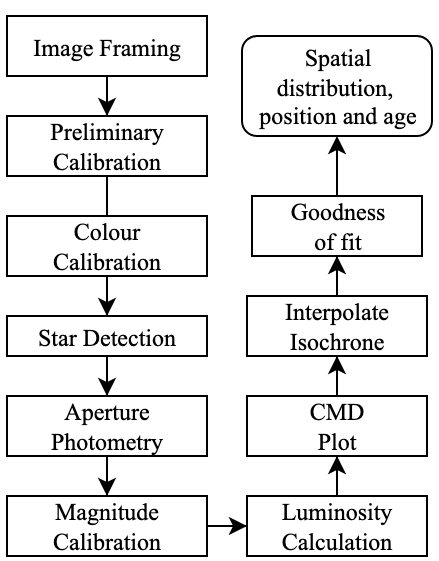
\includegraphics[width = 5cm]{figures/steps.png}
    \caption{Overview of steps to be carried out during data analysis. }
    \label{fig: steps}
\end{figure}

\section{Preliminary Calibration}
The conventional calibration will be carried out using flat and bias images as with all photometry. However, it is also important to consider the frame size and colour calibration. The use of the telescope at Calor Alto Observatory (CAO) for this project will make use of B, V and R filters, which means that only 50mm of the 100mm detector can be used. This leaves an observable 11' circular unvignetted frame that will need to be cropped before analysis using \verb|numpy.s_|. \\ This means that about a 10' by 10' area will be suitable for observation after the crop. This will limit the size of the open cluster that can be observed and will need to be taken into consideration when choosing targets. \\ Color calibration is not as important to consider throughout this study as it aims to be self-contained regarding colour comparison to both experimental and archived data. However, if colour calibration proves to be a necessary step, CAO is equipped with a filter wheel reference sheet along with reference targets. \footnote{\url{http://w3.caha.es/CAHA/Instruments/CAFOS/cafos22.html}} 

\section{Stellar Detection} \label{sec: stellar_detect}

Upon first observing open clusters, each member of the clusters must be first identified. After each target has been successfully framed and reduced photometry must be performed to identify each star. \\ This can be completed using \verb|DAOstarfinder| from the \verb|photutils| python module.\footnote{\url{https://github.com/astropy/photutils/tree/v0.3}} \\ This operates on the DAOFIND algorithm coined by \cite{DAO_PHOT}. When given a threshold value \verb|DAO| will search local density maxima for peaks that surpass this threshold. \verb|DAO| will then fit a 2D Gaussian kernel to find objects of similar shape and size. Furthermore, the applied Gaussian kernel can be used to find the centroid and roundness by marginally fitting a 1D distribution of the Gaussian kernel to the unconvolved data image. The important return of data from the star finder is the x and y centroid positions and roundness. \\ Once this is complete, it is then possible to continue on the path to magnitude calculation. For a comprehensive discussion of implementation and mathematical framework, see \cite[Ch. 5.1-5.3]{howell_2006} and \cite{DAO_PHOT}

\subsection{Selecting Detection Parameters}

The two important parameters that require attention is the \verb|threshold| and the \verb|FWHM|. 

I. The threshold determines what count number is considered the background and what count number is considered a star. \\ This value will depend on how noisy the image is so to ensure that they are no false detections the threshold expressed as follow, 

\begin{equation}
    \texttt{threshold} = 5 \cdot n_{\text{background}}
\end{equation}

II. The full width at half maximum (FWHM) of the Gaussian distribution defines the resolution of a point source. FWHM is the diameter of the star's image area where intensity has fallen by half its peak value. For accurate photometry at FWHM of at least two pixels is required. Where FWHM is initially taken to be 7 to find a hand full of stars. These stars can be fitted to a 2D Gaussian to find FWHM. The FWHM is updated accordingly, and the process is repeated until the desired result is attained. Where FWHM of distribution is expressed as, 

\begin{equation}
    \text{FWHM} = 2\sqrt{2 \ln(2)} \cdot  \sigma 
\end{equation}

\section{Instrumental Magnitude Calibration}
\subsection{Instrumental Apparant Magnitude Calaculation}

Next is the measurement of the brightness of each detected source. This is completed using \verb|aperture.photometry| from \verb|photoutils|\footnote{\url{https://photutils.readthedocs.io}}. The basic idea is that the counts measured can be directly related to magnitude. This is done by sampling a specified aperture area around each detected source along with taking the background counts around the source by defining the bounds of the annulus \citep{larry_bradley_2020_4044744}. 

\begin{figure}[h!]
    \centering 
    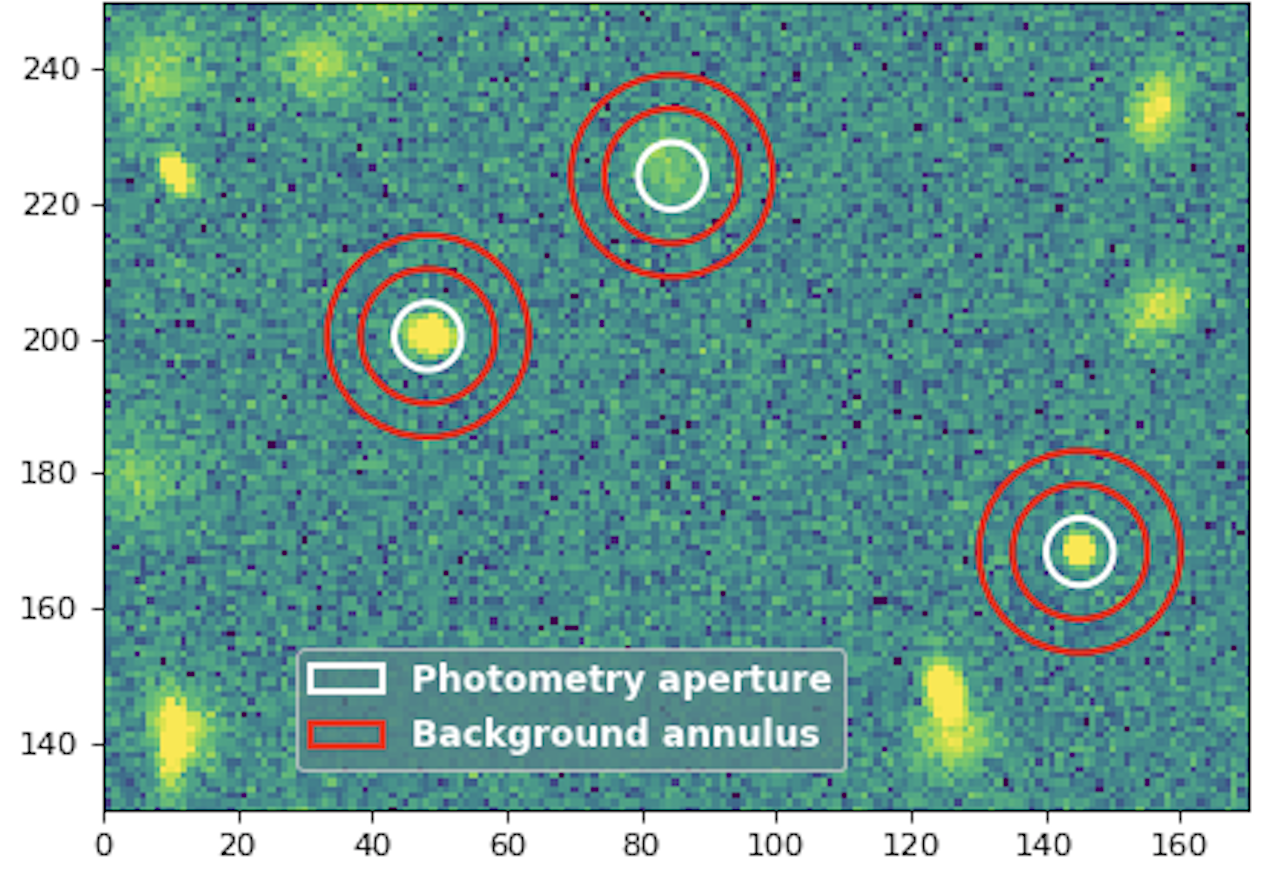
\includegraphics[width = 8cm]{aperture-1.png}
    \caption{Apertures using \texttt{photutils}. White circle is the aperture where the counts are summed and the red annulus is where the background counts are summed. Image curtsey of \cite{larry_bradley_2020_4044744}}
    \label{fig: aperture}
\end{figure}

The number of measured counts from \verb|aperture| photometry is related to magnitude as follows, 

\begin{equation}
    m_{\text{std}} = -2.5 \log_{10} F + \text{ZP}
    \label{eq: magnitude}
\end{equation}

Where $m_{\text{std}}$, is the calibrated magnitude of a given source in the \textit{standard} system. $F$, is the background-subtracted counts from a given source, and ZP is the zero point of an image. 

\subsection{Insturmental Conversion}

\Cref{fig: aperture} shows how \verb|aperture| handles the aperture and annulus. The aperture value is selected based on what aperture returns the lowest signal to noise ratio (SNR) during calibration. This is done by selecting a star from a frame and sampling other stars around it within a defined radius, i.e. 8 arcmins. This group of stars is then queried to a database (i.e. APASS\footnote{\url{https://www.aavso.org/apass}}). To return stars from the selected group with the most accurate astrometric values. The varying aperture values are used to see which returns the lowest SNR. A good guess value, in this case, would be the FWHM that was previously determined. The least noisy aperture will be returned and used for subsequent analysis. \\

The annulus will be selected based on where a uniform background count can be attained, usually around taken with the inner and outer boundary taken as 5 and 10 pixels extended outside the aperture. \\ In the case where there is an overlapping of stars, the background count can be taken from a sparsely populated region of the frame. This can be easily implemented using \verb|numpy.s_| and \verb|for| loops in tandem with source detection.   \\

Even though the magnitude of the sources can be calculated, they are only instrumentally apparent magnitudes. The next step is to covert each detected target into the standard photometric system. The purpose in this is to negate any discrepancies between the instrumental system and the standard system. This is done through the calculation of the zero point, ZP. \\ 

To find the zero-point, the use of reference stars is needed. A plot can be made between instrumental magnitude against the photometric magnitude to find the zero-point \cite[Ch. 6.1]{budding_o_2007} of the system, see \cref{fig: magnitude_test}. If done correctly, all-instrumental bias will be minimised. This procedure needs to be repeated for each filter used. 

\begin{figure}[h!]
    \centering
    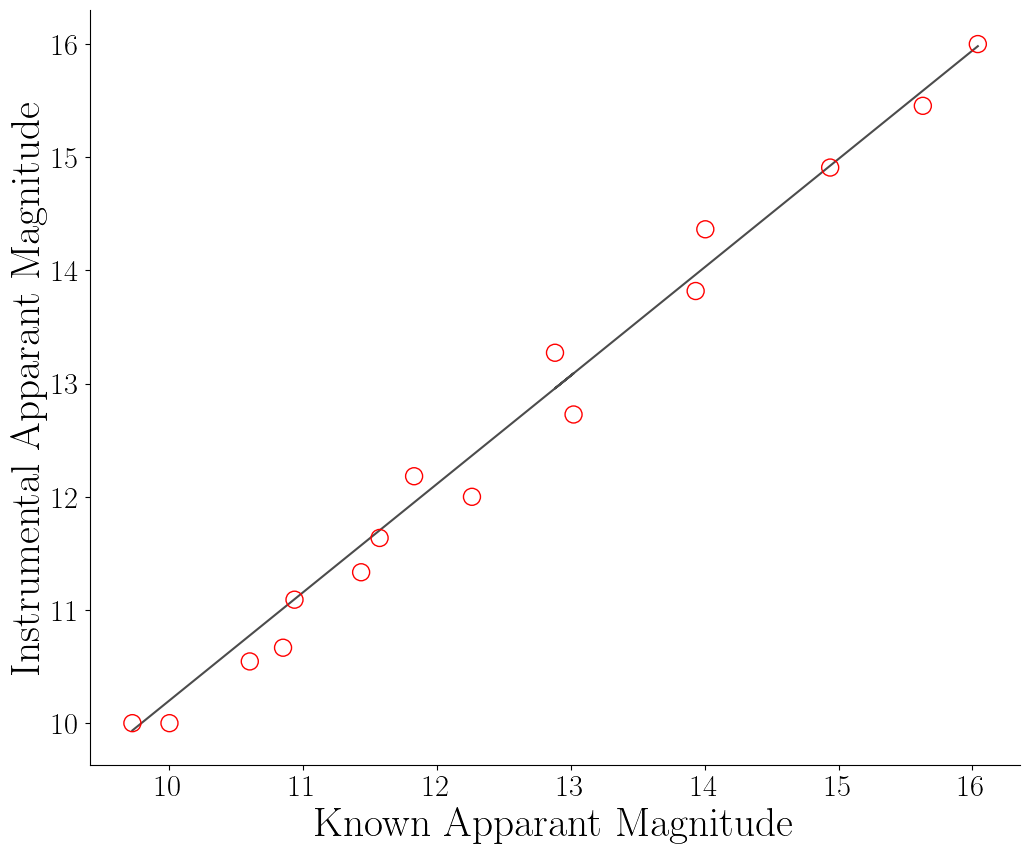
\includegraphics[width = 8cm]{figures/magnitud_calibration.png}
    \caption{Example plot of Magnitude calibration. Using provided data from NGC3286 and \texttt{astroquery} to use SIMBAD magnitude values.}
    \label{fig: magnitude_test}
\end{figure}

When the reference stars have been identified \cref{eq: magnitude} can be re-arranged to calculate the zeropoint,

\begin{equation}
    \text{ZP} = m_{\text{std}} + 2.5 \log_{10} F 
\end{equation}

\subsection{Statistical Uncertainty}

Photon's on a CCD obey a Poission distribution therefore before any measurements or analysis are made there is a built in uncertainty. This uncertainty is commonly referred to as signal to noise ratio (SNR). This is simply the signal from the detected star over the noise in the signal itself \citep[Ch. 5.3]{budding_o_2007}. Where it is expressed as follows, 

\begin{equation}
    n = n_{\text{aperture}}  \left( 1 + \frac{n_{\text{aperture}}}{n_{\text{annulus}}} \right)
\end{equation}

\begin{equation}
    \text{SNR} = \frac{S_{\text{star}}}{\sqrt{S_{\text{star}} +  n\left(S_{\text{bkg}}  \right)}}
\end{equation}

Where $n$ is respective area of pixels and $S$ is the respective photon count. This allows for an error estimation on magnitude to be expressed as follows, 

\begin{equation}
    \Delta m \sim \frac{1}{\text{SNR}}
\end{equation}

\subsection{Luminosity and Distance Calculations}

Following ZP being determined, the calculation of distance and luminosity can be determined using the following equations. 

\begin{equation}
    d = 10^{P}; \; \; \; P = \frac{5 - m_{\text{std}} - \text{ZP} }{5}
\end{equation}

Where luminosity can be calculated as follows, 

\begin{equation}
    L = 4\pi d^2 F
\end{equation}

An inquiry can also be made into the mass of main-sequence stars present in the stellar population if required by using the following equation. 

\begin{equation}
    L = L_\odot \left( \frac{m}{m_\odot}\right)^a \; \; \; \; (3 \lesssim a \lesssim 4) 
\end{equation}




\section{Colour-Magnitude Diagram} \label{sec: CMD-diagram}

Colour magnitude diagrams (CMD) are a variant of Hertzsprung-Russell (HR) diagrams. The HR diagram will summarise the temperatures against magnitudes of the stellar populations, whereas CMDs is magnitude against colour. CMDs are much easier to plot as the CMD does not require the temperature of each star in a cluster. Instead, the ratio of two spectral bands intensity is used. This ratio is directly related to the black body function and related to temperature. The balance is usually expressed as the magnitude difference between two optical spectral bands, i.e. B-V. This can be similarly expanded to flux as it is easier to plot and measure flux in a standard optical spectral band (usually V). Due to this reason, CMDs are used more commonly in cluster observation. See \cref{fig: CMD_plot} as an example. \\ 
Plotting a CMD is relativity easy once proper calibration of magnitudes for the required filters has been performed. It just requires the use of \verb|matplotlib|.  

\begin{figure}
    \centering
    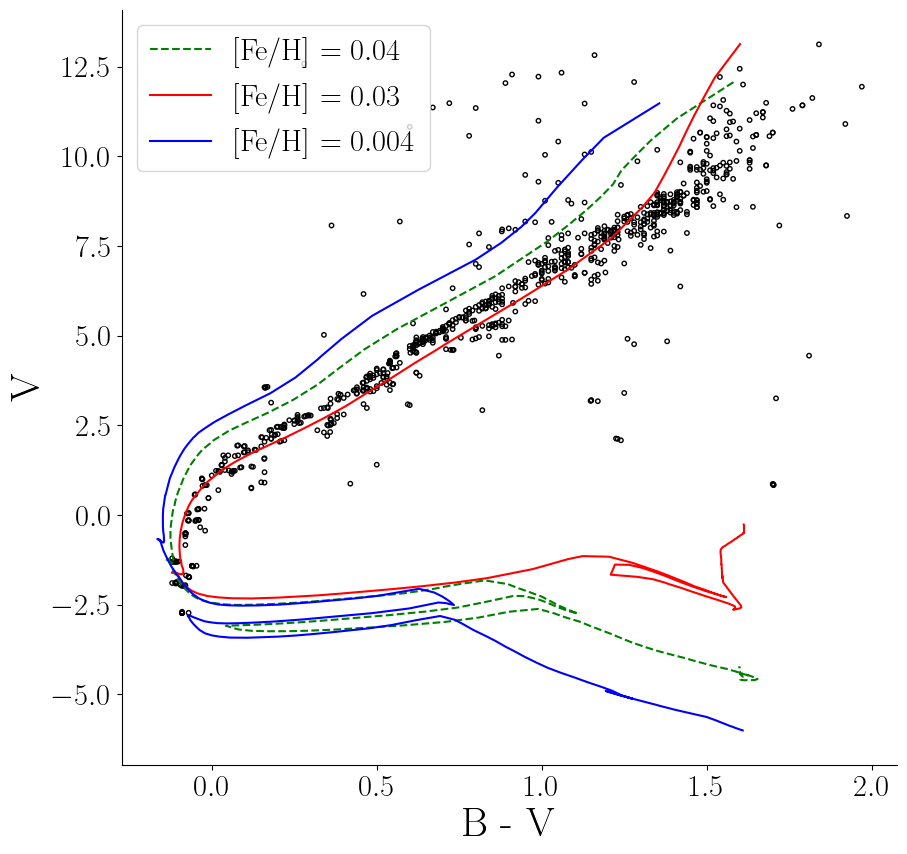
\includegraphics[width = 8cm]{figures/M45CMD.png}
    \caption{Example CMD plot of M45 using discussed methods using SIMBAD data. MIST isochrones were generated for a range of metallicities between $0.008 < [\text{Fe/H}] < 0.03$. 100 Myr fitted the data closely and parameters are within close range of \cite{1985_Vandenberg}. All mention packages and databases are used in the creation of this plot as a proof of concept.}
    \label{fig: CMD_plot}
\end{figure}

\section{Theortical Stellar Isochrone} \label{sec: Isochrone}

Once the CMD has been plotted, it is time to turn to fit a stellar isochrone. This part of the analysis is inferred from much of the information about a stellar population. There are a considerable amount of models for creating isochrones such as MIST\footnote{\url{http://waps.cfa.harvard.edu/MIST/references.html}} \citep{choi, PAXTON}. \\  

\verb|isochrone|\footnote{\url{https://isochrones.readthedocs.io/en/latest/}} can be used in tandem with MIST to quickly generate isochrones with varying parameters. This is done using the \verb|StarModel| object class, allowing tabulated pairs of varying parameters to be quickly downloaded in mass to a binary form using the \verb|grid| extension of \verb|starmodel|. \verb|isochrone| uses grid interpolation based on \verb|pandas| and \verb|scipy| modules to produce multi-indexed isochrone data frames at fast speeds. This allows for isochrone model generation and plotting in a more efficient way than a manual generation through MIST and ultimately will allow for a different range of parameters to be fitted due to ease of use and automation of interpolating process. 

\begin{table}[h!]
    \begin{tabular}{l r}
        \hline \hline 
        Parameter & Inferred from Photometry \\ \hline 
        RA (J2000) & YES \\
        DEC (J2000) & YES \\ 
        Galaxy Longitude & YES \\ 
        Galaxy Latitude &  YES \\ 
        Distance & YES \\ 
        Distance Modulus ($m_{std}$) & YES \\ 
        Age & YES \\ 
        Metallicity & ESTIMATED \\ 
        Reddening & ESTIMATED \\ \hline 
    \end{tabular}
    \caption{Required parameters in calculation of a MIST theortical isochrone. YES - can be directly inferred from observations. ESTIMATED - inferral is possible but will have to be compared with other databases.}
    \label{tb: parameters}
\end{table}


\subsection{Reddening}

Reddening is a direct result of propagation through the interstellar medium (ISM), causing light to diffuse. The extent of reddening is inversely proportional to the wavelength of the optical light. Reddening can be expressed as an excess of colour, $E(B - V)$ in a photometric system. With this absorption expressed as follows at a given wavelength, 

\begin{equation}
A_v = R_v \ E(B - V)
\end{equation}

Where $A_v$ is the adsorption value at $R_v$ is the degree of redding at a specific wavelength. Reddening will affect the stars' horizontal position when plotting the CMD as the diffuse through the ISM will decrease detected light. In correcting reddening, the loss of light will be taken into consideration. V-band adsorption, $R_v$, has been estimated to be $\sim 2.5$ towards the Milkey Way's bulge \citep{DAVID_M_Reddening}. However, this value changes based on the target position. Nevertheless, there are plentiful high-resolution spectroscopic studies to provide reliable estimations.

\subsection{Metallicity Esitmations} \label{sec: metallicity}
Metallicity proves to be quite useful when analysing open clusters as its it's a strong indicator to what stars are part of the stellar population in the cluster itself. Using discrepencies in magnitude along with comparison with metallicity 'imposter' stars can be idenitifed. However, metallicity primarly uses spectorscopy for accurate estimations, commonly analayesd through comparioson of the Sun using a log scale, 
\begin{equation}
    \left[ \frac{\text{Fe}}{\text{H}} \right] = \log_{10} \left[ \frac{\text{Fe/H}}{\text{Fe/H}}_\odot \right] 
\end{equation}
Using this scale, photometric colours can be used to estimate metallicity to a reasonable degree, as shown by \cite{kar} using U, V and B filters. However, this would require the use of narrowband filters for more significant periods of observation time to attain values equivalent to high-resolution spectroscopic databases such as \cite{Metallicity_catalogue}. 

\subsection{Convection Overshooting} \label{sec: convection_overshooting}

Convection overshooting has been shown to be a necessary consideration for stellar models which has been most notable shown by \cite{Overshooting_Vandenberg}. It is the also the reason why earlier stellar studies assumed that convection cores were enlarged at some given pressure height. When creating a mdoel convection cores should not exceed $r_{\text{max}}$. The maximum size of a convection core is given as follows as, 

\begin{equation}
    \int^{r_{\text{max}}} (L_{\text{rad}} - L) \frac{1}{T^2} \frac{dT}{dr} \; dr = 0 
\end{equation}

Successfully correcting for overshooting produced more accurate plots for the later stages in the main sequence as shown in \cref{fig: convection_overshooting}. Most theoretical isochrone models readily include convection overshooting as a parameter, thus making for easier implementation onto CMD plots. Inclusion will see better fits in the later main-sequence as shown by \cref{fig: convection_overshooting} and \cref{fig: CMD_plot}

\begin{figure}[h!]
    \centering
    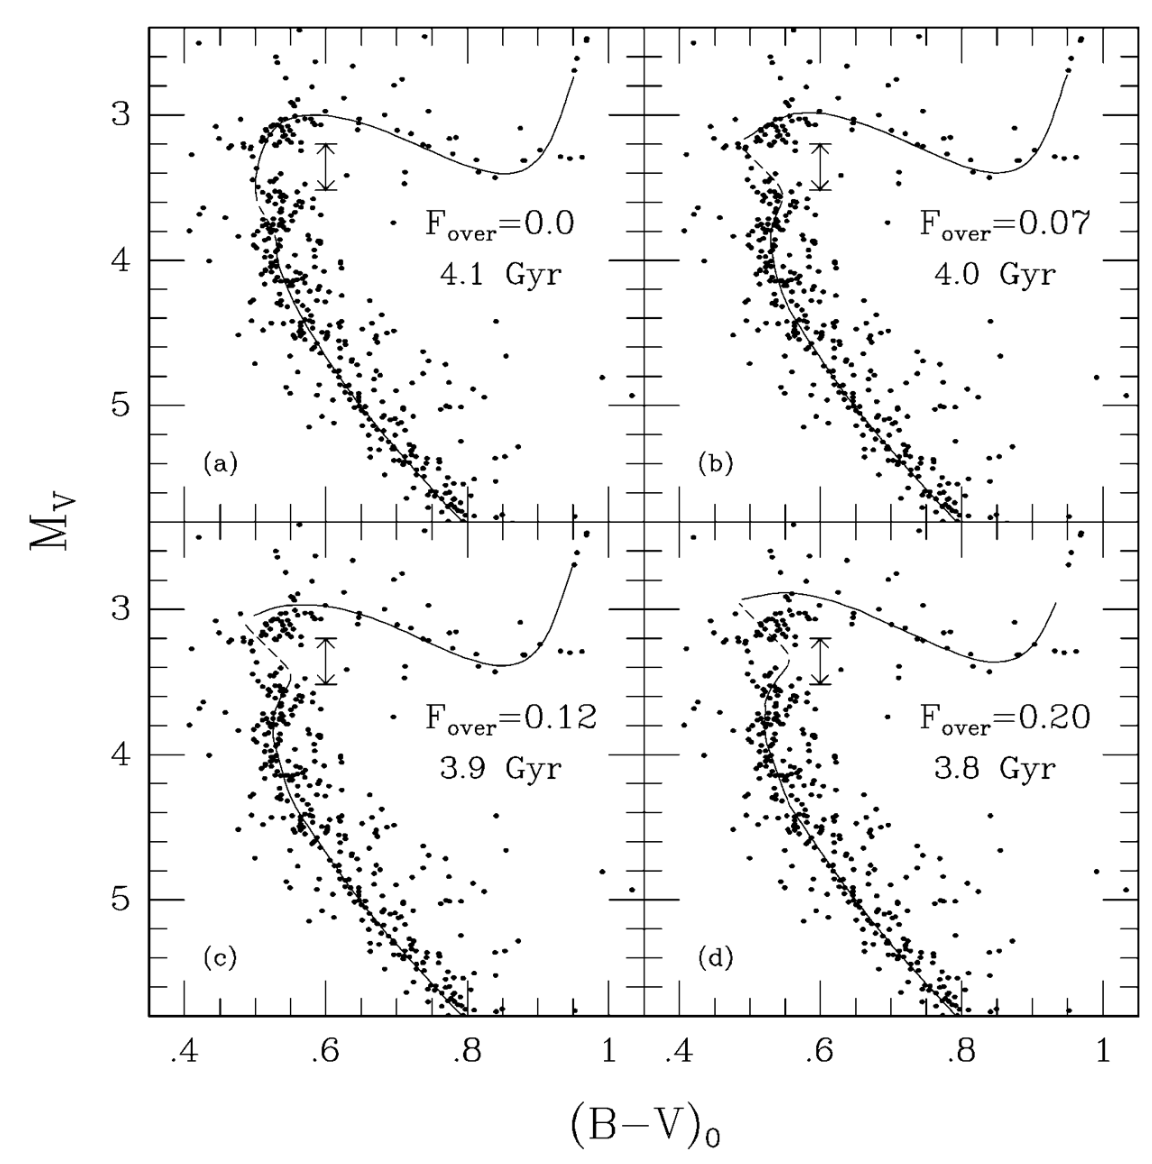
\includegraphics[width = 8cm]{figures/CMD_convectio_overshooting.png}
    \caption{Theortical isochrones fitted with varying values of age and overshooting, $F_{\text{over}}$ as shown by \textcite{1985_Vandenberg}}
    \label{fig: convection_overshooting}
\end{figure}

\section{'Goodness' of Isochrone Fit}

In fitting the isochrone to observed data also requires a tangible way to show that the isochrone is well fitted. This is important, especially when dealing with minor changes of the estimated parameters in \cref{tb: parameters}. Two developmental methods have been outlined by \cite{2006MNRAS.373.1251N} and \cite{GoodnessValle}, but there is no generally agreed-upon methodology when measuring the  'goodness' of fit. A chi-squared $(\chi^2)$ test can be performed using \verb|scipy| and easily implemented. The following expression can be used to perform the test, 

\begin{equation}
    \chi^2_c = \sum \frac{(O_i - E_i)^2}{E_i}
\end{equation}

Where $O$ is the observed value, and $E$ is the expected value. After each interpolation, the isochrone can be compared against the cluster data for each $i$th point taking $E_i$ to be the closest point on the isochrone. This will be taken as the $(O - E)^2/E$ component to be summed. The code suite created by \cite{2006MNRAS.373.1251N} runs quickly and provides similar results as produced in \cref{fig: CMD_plot} with much more rigour on how well the isochrone fits. However, interpolation of $F_{\text{over}}$ parameters does not appear to be implemented as of the most recent stable release. 

\section{OPen clusters home in the galaxy}

Finally, following the calibration of both magnitude and the theoretical isochrone, an estimation of age, distance, and spatial distribution can be made. Distance and age at this point will be calculated. Along with this any imposters in the stellar population will be removed if spotted as outliers during magnitude or metallicity calibration. From here, the cluster can be classified, and comments can be made on the stellar evolution of the cluster and evolution in both the galactic bulge and arms or any of the previously discussed parameters \citep{review}. 
